\section{Critical Review}
\captionsetup[figure]{font=small,labelfont=bf}
% Dit hoofdstuk is een opsomming van dat wat er al bekend is over het in de introductie beschreven onderwerp. Zeker bij practice based research gaat dit niet alleen om academische literatuur. Ook repertoire in de vorm van al bestaand werk, maakprocessen, contexten, technologieën, enzovoort is relevant, net als literatuur die niet strict academisch is zoals artikelen uit vakbladen, documentaires, enzovoort. In het critical review hoofdstuk wordt het eerder geïntroduceerde onderwerp in verband gebracht met relevante literatuur en repertoire.

% NOTES
% - Critical review naar bestaande media (Phonograph, LP, tape, CD, MP3, Torrent/P2P, Streaming)
% - Korte technische uitleg wat het is
% - Disruptieve werking van een medium op zijn voorganger
% - Welk probleem heeft het proberen op te lossen

% Inleiding
In dit critical review zal ik een deskresearch onderzoek doen naar bestaande media en diensten voor muziek distributie. Hierbij zal worden beschreven wat de disruptieve werking was van het medium ten opzichte van zijn voorganger en wat het probleem is wat het medium probeerde op te lossen. Tot slot zal worden beschreven waarom het medium relevant is voor dit Supportive Narrative en het onderliggende project, de NichePlayer.

% Uitleggen disruptief effect
Onder disruptieve werking versta ik het volgende. Nieuwe media worden vaak uitgevonden in een actie-reactie proces. In het oude medium blijkt na gebruik een tekortkoming te zitten, wat door middel van het nieuwe medium wordt opgelost. Dit proces is niet altijd intentioneel. Sommige innovaties in de geschiedenis hebben geleid tot een grotere hoeveelheid piracy, veranderingen in de muziek zelf, en hoe men er naar luistert. Positieve effecten zijn bijvoorbeeld het ontstaan van nieuwe genres.

\todo{Fact-checken van alle onderstaande uitspraken}

% ---------------------------------------------------------------------------------------- %
\subsection{Analyse bestaande media}
In dit onderzoek kan in theorie terug worden gegaan tot in de oudheid. Het doorgeven en distribueren van muziek is een onderdeel van cultuur, en daarmee iets wat ons mens maakt. Om een kaderen te stellen wordt gefocust op distributiemedia die klinkend geluid (i.e. geluidsgolven) dragen, beginnende bij de eerste, de fonograaf.

\subsubsection*{Fonograaf}
\begin{wrapfigure}{r}{0.25\textwidth}
    \centering
    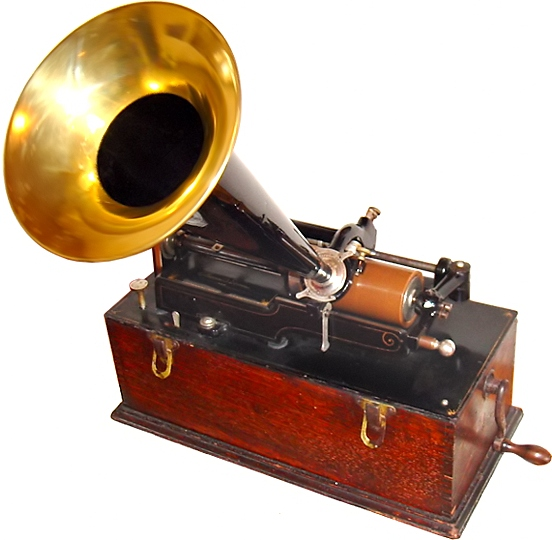
\includegraphics[width=0.25\textwidth]{critical-review/EdisonPhonograph.jpg}
    \caption{Fonograaf}
    \label{fig:critical-review:phonograph}
\end{wrapfigure}

% Beschrijving medium
De fonograaf (phonograph in Engels) is een van de eerste distributie media die het geluid zelf draagt ten opzichte van een beschrijving van de muziek. De geluidsgolven worden opgeslagen door met een naald in een wassen rol te krassen. De diepte van de kras staat gelijk aan de uitslag van het membraan. Tijdens het afspelen wordt het proces omgedraaid; een naald glijdt door de krassen en brengt hiermee het membraan in beweging. Het geluid wordt vervolgens versterkt door een hoorn.

% Klinkende muziek in huis zonder instrument
Door de uitvinding van de fonograaf werd het mogelijk om klinkende muziek in huis te hebben, zonder dat hier een instrument voor bespeeld hoefde te worden. \todo{Aanvullen}

% Alle soorten muziek beschikbaar
Hiermee is het dus ook mogelijk om een opname van een heel orkest af te spelen binnen huis, iets wat voor de uitvinding niet kon vanwege de ruimte.  \todo{Aanvullen}

% Minder focus op eigen interpretatie
Mensen konden hiermee ook 'perfecte' versies van de muziek beluisteren. In plaats van eigen interpretaties van bladmuziek wordt geluisterd naar een enkele uitvoering van een artiest. Niet alle aspecten van het bespelen van een instrument kunnen immers beschreven worden op papier, waardoor er altijd een eigen interpretatie wordt gespeeld door de muzikant.

% Beperking: maximale speeltijd
Een beperking ten opzichte van zijn de voorgangers is dat de fonograaf (en opvolgende iteraties) een maximale speeltijd hadden. Geschreven muziek kan in principe een oneindige lengte hebben. Het is dan ook interessant om te zien dat muziek zich is gaan aanpassen naar de mogelijkheden van het medium van zijn tijd.

% Relevantie NichePlayer
De Fonograaf is relevant in het onderzoek naar de NichePlayer omdat het een significante verandering bracht in de manier waarop mensen naar muziek luisterde en hoe het werd geschreven. Voor het eerst kon in de huiskamer van mensen met een gemiddeld inkomen naar perfecte uitvoeringen van muziek worden geluisterd. De NichePlayer probeert

\todo{Relevantie NichePlayer}

% NOTES
% - Opvolger op live muziek en zelf spelen
% - Muziek 'hoe het zou moeten klinken'
% - Redelijk goedkope manier om (klinkende) muziek in je huis te krijgen
% - Beperking in speeltijd

\subsubsection*{Grammofoon en iteraties}
\begin{wrapfigure}{r}{0.25\textwidth}
    \centering
    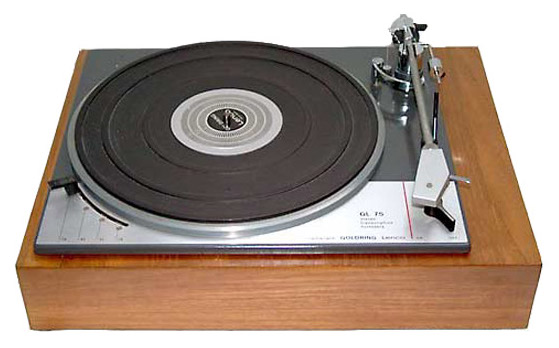
\includegraphics[width=0.25\textwidth]{critical-review/Gramaphone.jpeg}
    \caption{Gramaphone}
    \label{fig:critical-review:Gramaphone}
\end{wrapfigure}
De grammofoonplaat is een iteratie op de wasrol. In plaats van een ronde rol is het geluid bij de grammofoon opgeslagen op een platte plaat. Het schrijven en afspelen werkte bij de eerste iteraties van de grammofoon nog steeds voornamelijk mechanisch en per individuele plaat. In de latere iteraties van de grammofoonspeler werd meer electronica verwerkt waardoor de kwaliteit en volume van het geluid beter werd, massaproductie mogelijk werd en het daarnaast ook mogelijk werd om de muziek in stereo af te spelen.

Een groot voordeel van de grammofoon is het medium waarop de muziek is opgeslagen: een plaat ten opzichte van de wasrol. Platen zijn makkelijker te massa-produceren omdat ze gedrukt kunnen worden vanuit een mal. Een wasrol moet individueel worden beschreven en kan hierdoor niet makkelijk in grote hoeveelheid geproduceerd worden. Platen zijn daarnaast ook makkelijker in opslag omdat ze plat zijn. Door het gebruik van vinyl bij latere platen blijven ze ook langer goed.

Net als de wasrol heeft een plaat een maximale speelduur vanwege zijn formaat. Door technische restricties van verschillende soorten spelers zijn standaarden ontstaan voor de lengte van platen. De eerste generatie grammofoonplaten hadden door hun formaat (30cm, 12"), naalddikte en toerental van 78rpm een maximale speelduur van ongeveer 5 minuten. Het toerental komt voort uit een optimale geluidskwaliteit bij de afstand tussen de groeven van een 12" plaat, en het gebruik van standaard naainaalden. Door technische verbeteringen werd het vanaf 1950 mogelijk om platen met een speeltijd tot 40 minuten te drukken. 

Deze standaarden worden tegenwoordig nog steeds aangehouden, ondanks dat dit vanwege de nieuwe technologieën niet meer nodig is. Albums zijn tegenwoordig vaak nog steeds rond 40 minuten lang. Dit is een interessant gegeven omdat het laat zien dat de technische beperkingen van een medium de manier waarop muziek wordt geschreven kan beïnvloeden. De NichePlayer heeft als creatief platform het doel om juist geen beperkingen op te leggen aan de muziek die erop wordt gepubliceerd. Er is geen maximale lengte van een nummer of album, afgezien van de beschikbare opslagruimte van de server. Daarnaast wordt op veel plekken in het proces de vrije keuze van de artiest benadrukt.

Hoewel de technologie van vinyl spelers al lange tijd achterhaald is blijft het een populair medium. Volgens een onderzoek van de RIAA \cite{year_end_2022_RIAA_revenue_statistics} was de omzet van de verkoop van vinyl in de VS in 2022 hoger dan dat van de CD. Er werden dat jaar rond de 41 miljoen platen verkocht met een totale waarde van \$1.2 miljard dollar tegenover 33 miljoen CDs ter waarde van \$483 miljoen dollar. Het is opvallend dat vinyl een beter verkocht medium is in deze tijd. De CD qua geluidskwaliteit vele malen beter is dan vinyl, kleiner en makkelijker af te spelen.

% \todo{Relevantie NichePlayer}
% NOTES
% - [x] Na wasrol platte plaat van vinyl
% - [x] Vinyl makkelijker in opslag
% - [x] Vinyl makkelijker in (massa) productie
% - [x] Veel iteraties: langere platen, stereo, kwaliteit verbetering, etc.

\subsubsection*{Cassette}
\begin{wrapfigure}{r}{0.25\textwidth}
    \centering
    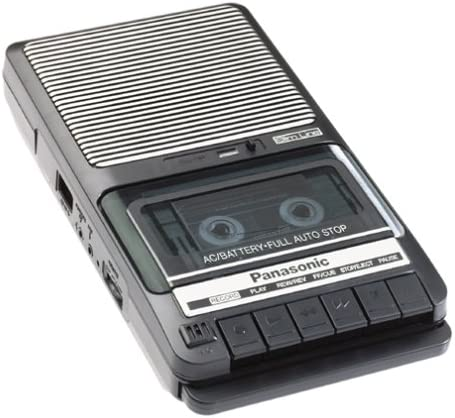
\includegraphics[width=0.25\textwidth]{critical-review/Tape.jpg}
    \caption{Cassette recorder}
    \label{fig:critical-review:tape}
\end{wrapfigure}
Bij de cassette is het geluid opgeslagen op een magnetisch geladen strip. De strip is opgerold in een plastic behuizing, een cassette, en kan worden afgespeeld met een speciale speler. De cassette speler rolt de strip af van de ene spoel naar de andere en leest de magnetische strip af met een leeskop. De signalen worden vervolgens versterkt en omgezet in geluid.

Een belangrijk voordeel van de cassette is dat het een medium is wat makkelijk meegenomen kan worden. De cassette is klein en gebruikt relatief eenvoudige technologie. Hierdoor is het mogelijk om een cassette speler te maken die op batterijen werkt, wat het vervolgens weer mogelijk maakt om muziek mee te nemen en af te spelen op plekken waar geen elektriciteit is. Dit is een groot voordeel ten opzichte van de platenspeler. De platenspeler is te groot en te zwaar om makkelijk mee te nemen.

Daarnaast is het ook mogelijk om zelf opnames te maken op een cassette. Het opnemen van muziek op een cassette is echter niet zonder kwaliteitsverlies. De magnetische strip is gevoelig voor ruis en de kwaliteit van de lees- en schrijfkop bepaald sterk de kwaliteit van het geluid. Het is niet mogelijk om een exacte kopie te maken van een cassette. Mensen konden zelf mixtapes maken van hun favoriete muziek, en deze vervolgens verdelen onder hun vrienden. Dit heeft een nieuwe cultuur gecreëerd rondom het medium die nog steeds zichtbaar is in sommige genres.

Het kunnen opnemen op een cassette tape is echter niet altijd een gewenste functionaliteit. Het is hiermee namelijk mogelijk om bestaande muziek op te nemen van de radio, plaat of van een andere cassette, zonder hier voor te betalen. Hiermee kunnen veel illegale kopieën worden gemaakt, ofwel piracy. \todo{Aanvullen}

% \todo{Relevantie NichePlayer}
Cassettes zijn interessant voor de NichePlayer vanwege hun effect op de cultuur van muziek. Het is een medium dat makkelijk te verspreiden is en waarop mensen zelf muziek kunnen opnemen. Dit principe zou ook in de NichePlayer verwerkt kunnen worden.

% - [ ] Kopiëren (met kwaliteitsverlies)
% - [ ] Nieuwe Cultuur, Mixtapes
% - [ ] Opnemen vanuit andere media zoals radio (piracy!)
% - [ ] Portable

\subsubsection*{CD}
\begin{wrapfigure}{r}{0.25\textwidth}
    \centering
    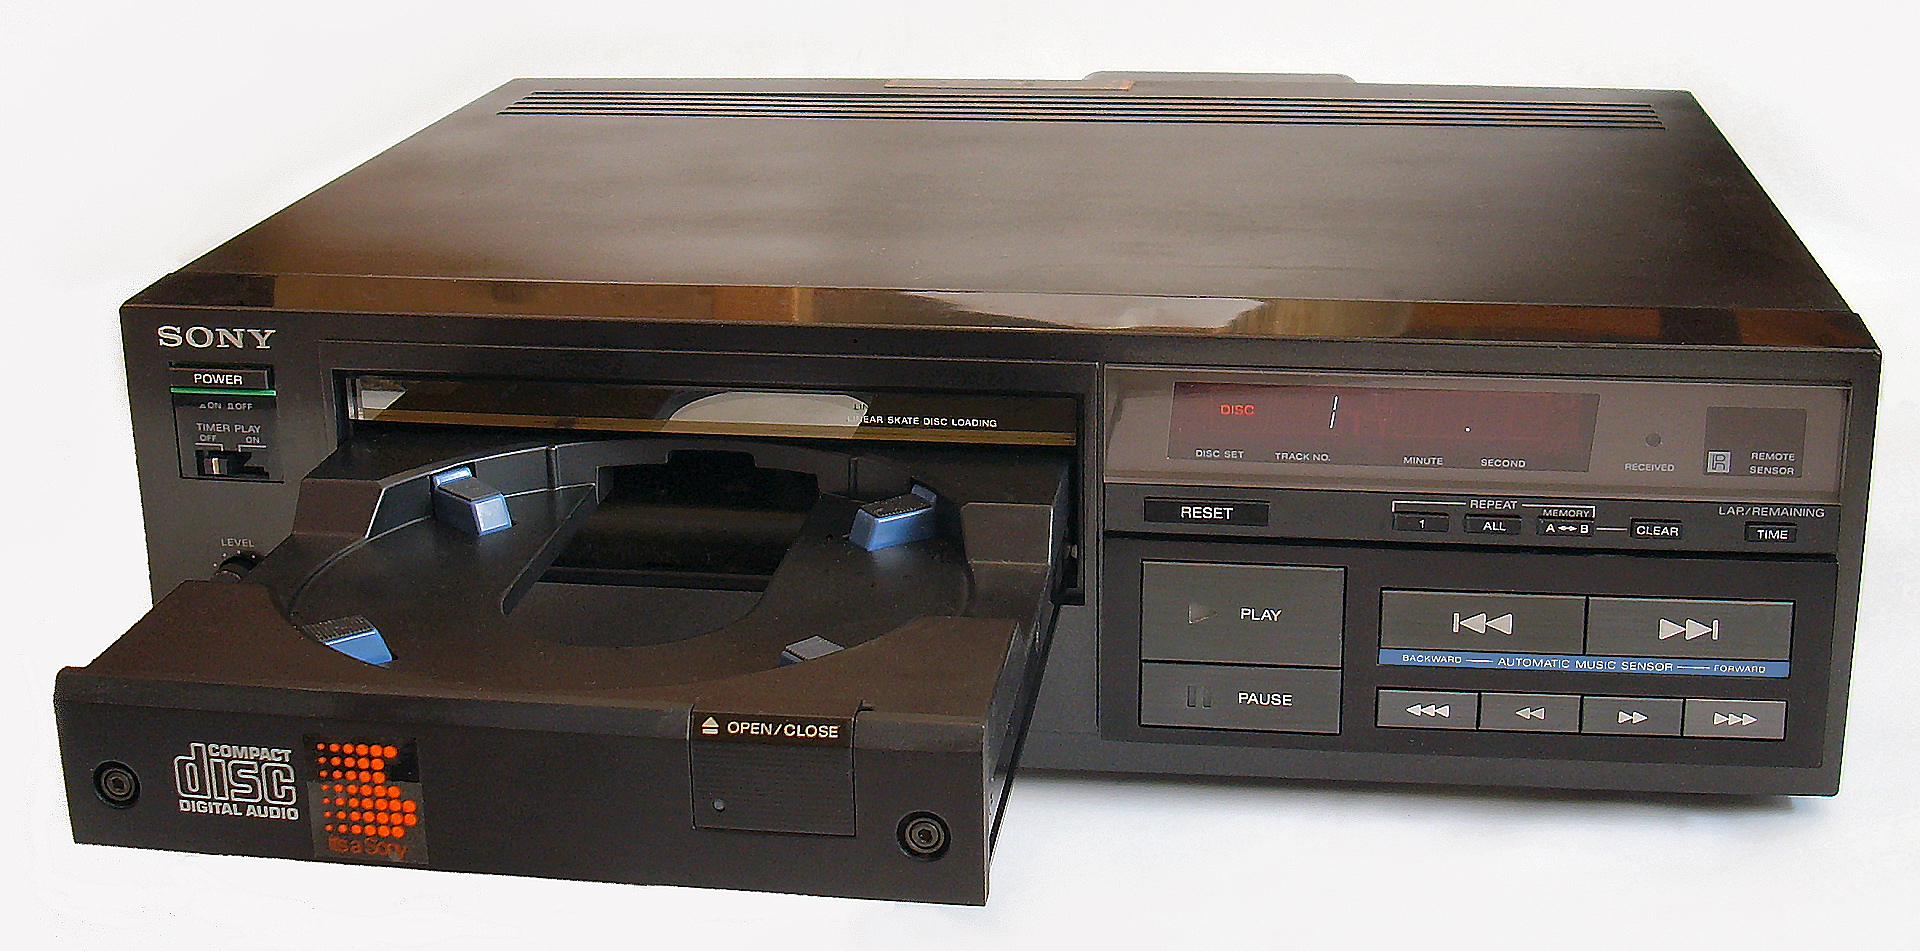
\includegraphics[width=0.25\textwidth]{critical-review/CD-Player.jpeg}
    \caption{Eerste commerciële CD speler}
    \label{fig:critical-review:cp-player}
\end{wrapfigure}
De CD is het eerste digitale medium. Net als de grammofoonplaat wordt het geluid opgeslagen op een schijf door middel van putjes. Bij een CD wordt echter geen gebruik gemaakt van een naald, maar wordt de diepte van de groef gelezen door een laser.

Het grote voordeel van de CD is de kwaliteit.

Daarnaast gaat de kwaliteit van CD's over lange tijd niet verloren.

\todo{Relevantie NichePlayer}

\begin{itemize}
    \item Hoge kwaliteit
    \item Geen kwaliteit verlies na lange tijd opslag
    \item Hoewel het populair was heeft niemand meer een speler (voordeel digitaal)
    \item Bootlegging
\end{itemize}

\subsubsection*{Internet}
\begin{wrapfigure}{r}{0.25\textwidth}
    \centering
    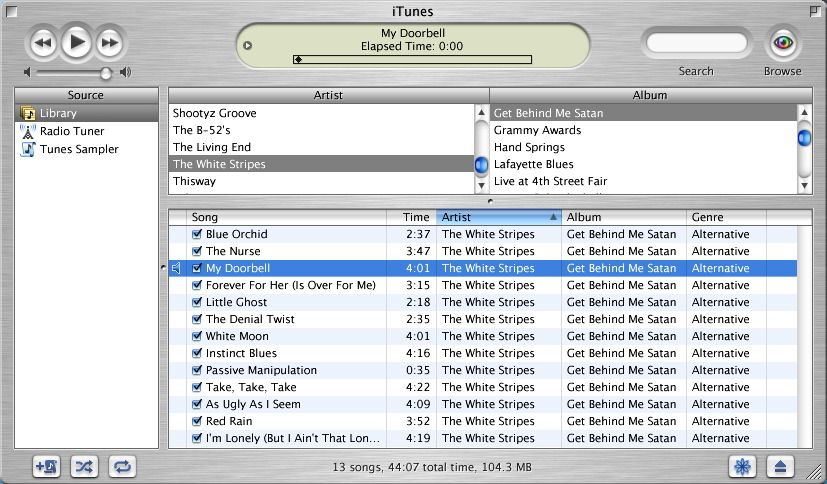
\includegraphics[width=0.25\textwidth]{critical-review/iTunes_v1.jpeg}
    \caption{iTunes}
    \label{fig:critical-review:iTunes}
\end{wrapfigure}

\todo{Relevantie NichePlayer}

\begin{itemize}
    \item Alleen mogelijk door opkomst MP3 en andere compressie formats
    \item iTunes \begin{itemize}
        \item Legale toegang
        \item Betalen per nummer
    \end{itemize}
    \item Torrents en Peer2Peer \begin{itemize}
        \item Illegale toegang
        \item Tegenreactie op iTunes
        \item Lang wachten voor kwaliteit
    \end{itemize}
    \item Onbeperkt kopiëren zonder kwaliteitsverlies
    \item Directe toegang tot meer muziek (fysiek gezien ten opzichte van CD's)
\end{itemize}

\subsubsection*{Streaming}
\begin{wrapfigure}{r}{0.25\textwidth}
    \centering
    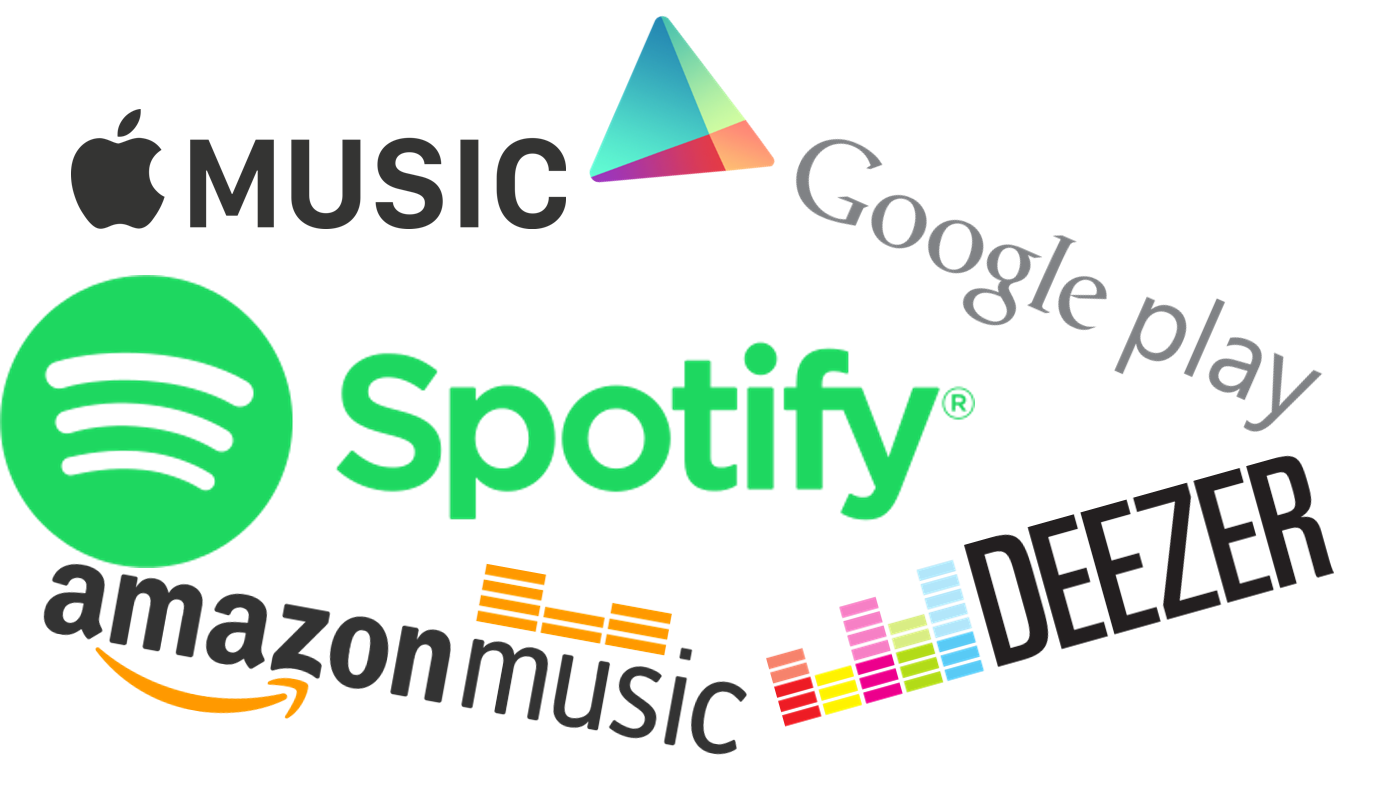
\includegraphics[width=0.25\textwidth]{critical-review/StreamingServices.png}
    \caption{Streaming services}
    \label{fig:critical-review:StreamingServices}
\end{wrapfigure}

\todo{Relevantie NichePlayer}

\begin{itemize}
    \item Legale, onbeperkte toegang
    \item Ander luistergedrag: \begin{itemize}
        \item Album minder belangrijk dan playlists
        \item Drop uitgesteld tot na 1:00 ivm betaling
    \end{itemize}
    \item Meer muziek als singles
    \item Alleen mogelijk door groei internet
\end{itemize}

% ---------------------------------------------------------------------------------------- %
\subsection{Concurrerende projecten}
\subsubsection*{TapTapes}
\begin{wrapfigure}{r}{0.25\textwidth}
    \centering
    
\includegraphics[width=0.25\textwidth]{critical-review/TapTapes.png}
    \caption{TapTapes}
    \label{fig:critical-review:TapTapes}
\end{wrapfigure}
De NichePlayer is niet alleen in zijn soort. Er zijn veel vergelijkbare producten die het in de inleiding benoemde probleem proberen op te lossen. Een van deze diensten is TapTapes, een start-up uit Saarbrücken, Duitsland. Toevallig is dit het bedrijf waar ik in mijn bachelor stage heb gelopen. Het concept van de NichePlayer bestond toen al enkele jaren, maar heeft door de stage meer vorm gekregen.

TapTapes is een commercieel bedrijf die een dienst aanbiedt om muziek te luisteren waarbij toegang wordt gegeven met een fysieke kaart. Net als de NichePlayer moet deze kaart gescand worden door een telefoon om te koppelen aan het apparaat.

Het grote verschil tussen TapTapes en de NichePlayer is dat bij de TapTapes een overeenkomst tussen de artiest en TapTapes nodig is. TapTapes drukt namelijk de kaarten  en koppelen deze met het systeem voor beveiligde toegang. Daarnaast moet de software momenteel door TapTapes ingericht worden wat betreft uiterlijk en inhoud. Dit is een groot verschil met de NichePlayer, waarbij de artiest zelf de kaarten kan maken en de muziek kan koppelen. In het basis pakket van de NichePlayer ben ik als bedrijf zelfs helemaal niet betrokken, en kan de artiest alles zelf doen. Het businessmodel van de NichePlayer is gebaseerd op het aanbieden van extra diensten.

\todo{Aanvullen}

\subsection{NichePlayer}
\begin{wrapfigure}{r}{0.25\textwidth}
    \centering
    
\includegraphics[width=0.25\textwidth]{critical-review/NichePlayer.png}
    \caption{NichePlayer}
    \label{fig:critical-review:NichePlayer}
\end{wrapfigure}

% - Korte geschiedenis van de NichePlayer (vorige iteraties)
Er zijn in de afgelopen jaren veel iteraties geweest van de NichePlayer. Waar de ontwikkeling in 2014 begon als een simpele muziek player voor eigen gebruik (ik had toen geen Spotify maar wel een enorme muziek bibliotheek) is het nu uitgegroeid tot een product dat door iedereen te gebruiken moet gaan zijn. Het ontwikkelen van de NichePlayer is de rode draad geweest van mijn programmeer ontwikkeling. In iedere iteratie is mijn groei op het gebied van software development duidelijk te zien. Waar ik in de eerste iteraties alles zelf ontwikkelde ben ik later overgegaan naar het gebruik van libraries en frameworks. Ook is de code steeds beter georganiseerd en is de kwaliteit steeds beter geworden.

De NichePlayer is een streamingdienst wat speciaal wordt ontworpen met creativiteit, openheid en transparantie in gedachte. Door de NichePlayer te gebruiken krijgt de artiest controle terug over het medium in de vorm van inkomsten en layout. De gebruiker krijgt de mogelijkheid om de artiest te steunen door middel van fysieke verkoop gekoppeld aan toegang tot de muziek. 
De NichePlayer is ontwikkeld voor kleine en beginnende artiesten. De NichePlayer zal dan niet gaan concurreren met bestaande diensten, simpelweg omdat deze concurrentie niet kan worden gewonnen.

\subsubsection*{Laatste iteratie (Bachelor SN)}
De laatste significante iteratie van de NichePlayer was ontwikkeld als afstudeer project van mijn bachelor Muziek en Technologie. Bij deze versie gebruikte ik voor het eerst een backend framework (Symfony) en een frontend framework (VueJS). Dit was een grote stap voorwaarts in de ontwikkeling van de NichePlayer. Het gebruik van deze frameworks zorgde ervoor dat de code beter georganiseerd was en dat de ontwikkeling sneller ging. Het supportive narrative van mijn bachelor heb ik daarbij voornamelijk gebruikt om mijn proces te beschrijven en de keuzes voor technologieën te verantwoorden.

De rede dat dit niet de laatste iteratie is geworden voor productie is omdat het systeem softwarematig niet goed werkte. Het was niet mogelijk om met meer dan twee gebruikers tegelijk naar muziek te luisteren. De API werd niet correct aangeroepen en was daarbij ook niet goed geconfigureerd waardoor deze erg traag werkte. Ik gebruikte zelf ontwikkelde code om de frontend en de backend te laten communiceren en maakte niet gebruik van software technieken als relational mapping, caching en server-side filtering. Voor een prototype was dit geen probleem, maar voor een productie versie moet een systeem stabiel zijn en snel werken.

Daarnaast was de plek waar het systeem draaide een grote bottleneck. De backend draaide volledig in een virtuele server met weinig optimalisatie, en de data moest door verschillende computers heen om uiteindelijk bij de gebruiker te komen. Dit zorgde ervoor dat de backend niet goed bereikbaar was en dat de API niet goed werkte.

\subsubsection*{Nieuwe iteratie noodzakelijk}
% - Verschil met vorige iteraties NichePlayer, waarom was een nieuwe iteratie nodig?
Deze hiervoor genoemde problemen konden niet meer worden opgelost binnen de bachelor iteratie omdat het voornamelijk aan de core van het systeem lag. Daarom heb ik besloten om een nieuwe iteratie te starten waarbij deze problemen worden opgelost. Het concept blijft hierbij hetzelfde, en ook de libraries van de back- en frontend worden hergebruikt. Er worden echter wel nieuwe plugins toegevoegd waaronder een Object Relation Mapping plugin en een plugin voor communicatie met de API. De code wordt opnieuw geschreven volgens moderne syntax standaarden en geforceerd door binnen mijn code editor door middel van ESLint.

Object Relation Mapping is een manier om data aan elkaar te koppelen. Een gebruiker heeft bijvoorbeeld meerdere albums, en een album heeft meerdere nummers. Door gebruik te maken van ORM hoeft de programmeur niet zelf de data aan elkaar te koppelen, maar wordt dit automatisch gedaan. Dit zorgt ervoor dat de code minder complex is en dat er minder fouten gemaakt kunnen worden. Daarnaast is het met een ORM plugin makkelijker om een relatieveld van een object op te vragen (bijvoorbeeld het album van een nummer).
